\chapter{Method of Approach} 
\label{ch:methodofapproach}

This section has been broken down into two parts that each detail how each of the main composer components were developed.  The first section describes the processes and tools needed to develop the composer and the second section describes the processes and ideas behind the development of the user interface.

\section{Computer Composer Development}
\label{sec:computercomposerdevelopment}

To begin this project, it was necessary to develop the composer which would function as the backend of the tool.  This was chosen as the first step because the elements of the user interface would have to be chosen and designed based on what the composer was capable of doing.  Without first implementing the basic functionalities of the composer, it would be impossible to determine how the user interface should be built.  To develop the functions of the composer, several preexisting python tools and libraries were employed.

\vspace{\baselineskip}

\subsection{Tools}
\label{subsec:tools}

The following table lists all of the tools that were used and their specific functions within the composer.  None of these tools, on their own, where capable of forming the functioning composer.  Several of these tools have very advanced sets of functions, but no single tool had all of the required functions for the composer.

\begin{table}[!htbp]
	\centering
	\caption{Tools and packages and their uses in this project}
	\begin{tabular}{|l|l|}
		\hline
		LilyPond & Notation \\ \hline
		mingus & MIDI File Generation \\ \hline
		MIDIjs & Playback \\ \hline
		music21 & Melody Analysis \\ \hline
	\end{tabular}
\end{table}

\subsubsection{LilyPond}
\label{subsubsec:lilypond}

The primary function of LilyPond is as a text-based music engraving tool \cite{LilyPond_2020}.  LilyPond can either be used with a graphical user interface or as a command line tool by interfacing with another program \cite{LilyPond_2020}.  For the purpose of this tool, the command line version is being used by interfacing with mingus.

\vspace{\baselineskip}

This tool was chosen for this project due to its ease of integration and because of its ability to output high quality notation.  Additionally, the notation generated by LilyPond is easily customized and extremely flexible.  There are many options for editing the layout and spacing of the notation easily within the command line.

\vspace{\baselineskip}

To use LilyPond with the command line, the user must generate a text file.  The tools then uses the data in this file to draw the notation in the desired format.  For this tool, the text file is generated in the background as the user chooses notes and durations.  Then, the notation is drawn into an image that is displayed on the page.  A sample of the text file and the associated output is shown below.

\begin{figure}[!htbp]
	\centering
	\caption{LilyPond Text File and Output Example \cite{LilyPond_2020}}
	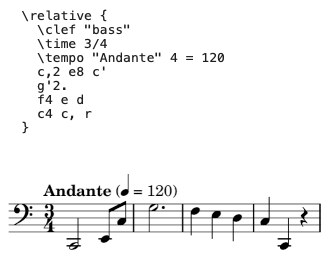
\includegraphics[scale=0.75]{images/lilypondExample.png}
\end{figure}

The \code{\textbackslash relative} in the text file has to deal with octave designation.  Adding \code{\textbackslash relative} sets each previous note as the center pitch and determines the octave of the following note to be the closest instance of that pitch either up or down.  Adding the \code{\textquotesingle} specifies how many octaves higher the note should be from the center pitch and adding the \code{,} specifies how many octaves lower it should be from the center pitch.  The number of \code{\textquotesingle}'s or \code{,}'s added is the number of octaves to shift the pitch.  The \code{\textbackslash clef}, \code{\textbackslash time}, and \code{\textbackslash tempo} indications refer to exactly for which they are named.

\vspace{\baselineskip}

In terms of pitch and duration content, the pitch is given by the letter name and duration is given by the number.  \code{1} for whole note, \code{2} for half note, \code{4} for quarter note, etc.  The \code{.} specifies whether or not that duration is meant to be dotted.  Finally, the \code{r} specifies a rest.

\vspace{\baselineskip}

Also important to note, the spacing within the lines of the text file and the newlines themselves are not taken into account by LilyPond.  These are simply for readability and are not required to generate the notation.  It appears as though the barlines may have been created this way, but are actually added automatically based on the meter signature.

\subsubsection{mingus}
\label{subsubsec:mingus}

mingus is a package for Python that provides advanced music theory and notation functions \cite{Spaans_2015}.  For this project, it is being used to generate MIDI files to be used later in playback and to interface with LilyPond to generate music notation.

\vspace{\baselineskip}

This tool was chosen for this project due to its ease of use and flexibility when generating files.  It has many functions that make it useful that are beyond the scope of this project, but in terms of creating MIDI files, it has the most direct method of doing this among similar tools.

\vspace{\baselineskip}

In order to generate a MIDI file, a NoteContainer must be created first.  This is quite simple to do in mingus.  After this step, there is a function that turns the NoteContainer into a MIDI file.  An example of this is shown below.

\begin{figure}[!htbp]
	\caption{mingus MIDI File Generation \cite{Spaans_2015}}
	\code{> nc = NoteContainer(["A", "C", "E"])} \\
	\code{> MidiFileOut.write\textunderscore NoteContainer("test.mid", nc)} \\
\end{figure}

Along with creating the MIDI files for playback, mingus also handles the interface with LilyPond in order to generate music notation.  The following example shows the process of building a bar in music with specific notes and then converting that bar into an image file that contains the notation.

\begin{figure}[!htbp]
	\caption{mingus LilyPond Notation Image File Generation \cite{Spaans_2015}}
	\code{> b = Bar()} \\
	\code{> b + "C"} \\
	\code{> b + "E"} \\
	\code{> b + "G"} \\
	\code{> b + "B"} \\
	\code{> bar = LilyPond.from\textunderscore Bar(b)} \\
	\code{> LilyPond.to\textunderscore png(bar, "my\textunderscore first\textunderscore bar")} \\
	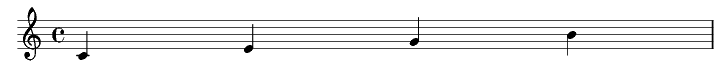
\includegraphics[scale=0.75]{images/mingusExample.png}
\end{figure}

\subsubsection{MIDIjs}
\label{subsubsec:midijs}

MIDIjs is a JavaScipt MIDI player that works with all modern browsers and is built entirely with JavaScript \cite{MIDIjs_ND}.  This tools was chosen for this project due to its high sound quality and ability to run without requiring any sort of download.  It runs in place and requires no plugins or extensions \cite{MIDIjs_ND}.  The following example shows how to play a MIDI file using MIDIjs.

\begin{figure}[!htbp]
	\caption{MIDIjs MIDI File Playback \cite{MIDIjs_ND}}
	\code{<script type=\textquotesingle text/javascript\textquotesingle  src=\textquotesingle //www.midijs.net/lib/midi.js\textquotesingle ></script>} \\
	\code{ <a href="\# " onClick="MIDIjs.play(\textquotesingle file.mid\textquotesingle );">Play file.mid</a>} \\
	\code{ <a href="\# " onClick="MIDIjs.stop();">Stop MIDI Playback</a>} \\
\end{figure}

\subsubsection{music21}
\label{subsubsec:music21}

music21 is a Python tool for computer analysis of music and musical data \cite{Cuthbert_2020}.  It is capable of analysis of large and small works alike with analytical categories such as harmony, form, structure, pitch content, rhythmic content, lyric content, frequency, intervals, and couterpoint.  It is capable of performing roman numeral analysis and generating post-tonal matrices.  In this project, music 21 is responsible for melodic analysis and providing the data to display feedback to the user on how to improve their melody.

\vspace{\baselineskip}

music21 was chosen for this project due to its deep and extensive analytical tools.  It is capable of powering all of the chosen elements of melodic analysis to assist the user during composition.  Several of the functions that are used within the feedback system are demonstrated below.

\vspace{\baselineskip}

This first example demonstrates how music21 is capable of checking for consonances and dissonances between pitches.  A starting and ending pitch are given and the function returns true if the interval is consonant and false if it is dissonant.  Intervals that are considered consonant by music21 are major or minor thirds or sixths, perfect fifths, and unisons.

\begin{figure}[!htbp]
	\caption{music21 Consonant Interval Checking \cite{Cuthbert_2020}}
	\code{> i1 = interval.Interval(note.Note(\textquotesingle C\textquotesingle ), note.Note(\textquotesingle E\textquotesingle ))} \\
	\code{> i1.isConsonant()} \\
	\code{True} \\
	\code{> i1 = interval.Interval(note.Note(\textquotesingle B-\textquotesingle ), note.Note(\textquotesingle C\textquotesingle ))} \\
	\code{> i1.isConsonant()} \\
	\code{False} \\
\end{figure}

This next example shows how music21 can identify the interval between two pitches.  The starting and ending notes are specified and a function is used to display the interval between them.  If \code{simpleName} is used, the interval is reduced to less than an octave.  If \code{semiSimpleName} is used, the interval is reduced to no more than an octave.

\begin{figure}[!htbp]
	\caption{music21 Interval Identification \cite{Cuthbert_2020}}
	\code{> n1 = note.Note(\textquotesingle c3\textquotesingle )} \\
	\code{> n2 = note.Note(\textquotesingle c5\textquotesingle )} \\
	\code{> aInterval = interval.Interval(noteStart=n1, noteEnd=n2)} \\
	\code{> aInterval.name} \\
	\code{\textquotesingle P15\textquotesingle } \\
	\code{> aInterval.simpleName} \\
	\code{\textquotesingle P1\textquotesingle } \\
	\code{> aInterval.semiSimpleName} \\
	\code{\textquotesingle P8\textquotesingle } \\
\end{figure}

This last example demonstrates how music21 can provide a pitch based on a starting pitch and an interval.  Once the starting pitch and the interval are given, a function can be used to return a new pitch based on a transposition of the first pitch.

\begin{figure}[!htbp]
	\caption{music21 Find Second Note Based on Interval \cite{Cuthbert_2020}}
	\code{> p1 = pitch.Pitch(\textquotesingle A\# 4\textquotesingle )} \\
	\code{> i = interval.Interval(\textquotesingle m3\textquotesingle )} \\
	\code{> p2 = i.transposePitch(p1)} \\
	\code{> p2} \\
	\code{<music21.pitch.Pitch C\# 5>} \\
\end{figure}

Later in the document, it will be shown how each of these functions were used to generate recommendations for how the user can improve their melody.

\pagebreak

\subsection{Main Composer Process}
\label{subsec:maincomposerprocess}

The following diagram shows the composition process broken down into the specific actions of the computer and the user.  While the user is responsible for more actions than the computer, the user is assisted in the process by the specific design of the interface and the directions that are provided when using the composer.  The computer then assists the user with melodic analysis to verify the quality of the melody in practical music theory terms.

\begin{figure}[!htbp]
	\centering
	\caption{Composition Process Flowchart}
	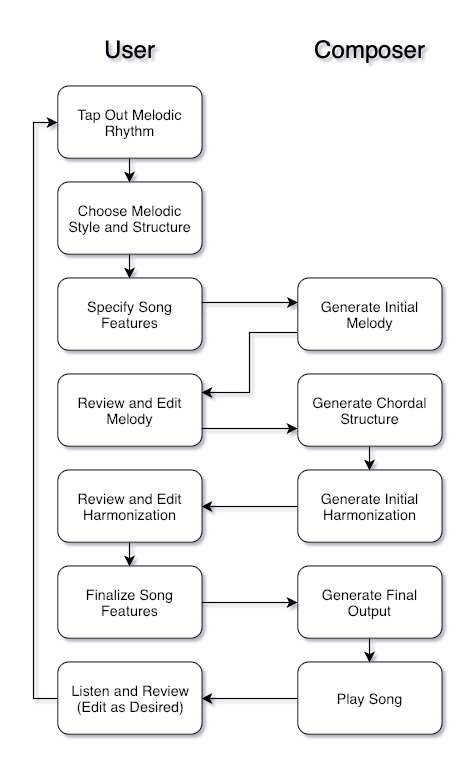
\includegraphics[scale=0.66]{images/composerProcess.png}
\end{figure}

\pagebreak

There are several important attributes that the user must choose when first creating their melody.  The following table lists each of these elements and their definitions in the context of this tool.  It is important to note that none of these values are final and they can be changed at any time.

\begin{table}[!htbp]
	\centering
	\caption{Melody Initialization Attributes}
	\begin{tabular}{|l|l|}
		\hline
		Base Note Duration & Base unit for time measurement and division \\ \hline
		Beats Per Minute & Number of base units per minute \\ \hline
		Beats Per Bar & Number of base units in each measure of music \\ \hline
		Total Number of Notes & Number of notes in the melody \\ \hline
		Note Set & Set of pitches available within the user's chosen key \\ \hline
	\end{tabular}
\end{table}

\subsubsection{Base Note Duration}
\label{subsubsec:basenoteduration}

In the context of this tool, this base note duration functions as the beat unit.  In music theory, the beat unit is defined as the note duration that gets on beat.  This is the bottom number in a meter signature.  The user has the option to select 2, 4, 8, or 16 as the base duration.

\subsubsection{Beats Per Minute}
\label{subsubsec:beatsperminute}

In the context of this tool, tempo is represented as the number of beats that occur per minute.  This aligns with the standard definition of tempo as the rate at which beats pass.  The duration that defines the beat in this tool is what the user selected as the base note duration.

\subsubsection{Beats Per Bar}
\label{subsubsec:beatsperbar}

To finish out the creation of the meter signature, the user must select the number of beats that will occur in each measure of music.  The user is not limited to any specific values here.  They can have as many or as few beats per bar as they desire.  In terms of the meter signature, this is the top number.

\subsubsection{Total Number of Notes}
\label{subsubsec:totalnumberofnotes}

Before the user begins to input notes, they must choose how many note entry forms that they want to render into the interface.  This number can be chosen arbitrarily as there is a good chance that they will not know the exact number that they want.  If this value is changed, the extra notes will be removed from the end.

\subsubsection{Note Set}
\label{subsubsec:noteset}

In the context of this tool, the note set is effectively the key signature.  The user will initially choose a starting pitch and a mode.  This will then define the set of notes that are available for the user to choose within the composer.  By limiting the notes to a particular key, this helps the user to be able to compose more coherent melodies.  It is also possible to manually add an accidental to any note.  The available accidentals are double flat \musDoubleFlat, flat \fl, natural \na, sharp \sh, and double sharp \musDoubleSharp.  The following note sets are available within the composer:

\begin{table}[!htbp]
	\centering
	\caption{Available Note Sets}
	\begin{tabular}{|l|l|}
		\hline
		C\fl Major & C\fl D\fl E\fl F\fl G\fl A\fl B\fl \\ \hline
		G\fl Major & G\fl A\fl B\fl C\fl D\fl E\fl F \\ \hline
		D\fl Major & D\fl E\fl F G\fl A\fl B\fl C \\ \hline
		A\fl Major & A\fl B\fl C D\fl E\fl F G \\ \hline
		E\fl Major & E\fl F G A\fl B\fl C D \\ \hline
		B\fl Major & B\fl C D E\fl F G A \\ \hline
		F Major & F G A B\fl C D E \\ \hline
		C Major & C D E F G A B \\ \hline
		G Major & G A B C D E F\sh \\ \hline
		D Major & D E F\sh G A B C\sh \\ \hline
		A Major & A B C\sh D E F\sh G\sh \\ \hline
		E Major & E F\sh G\sh A B C\sh D\sh \\ \hline
		B Major & B C\sh D\sh E F\sh G\sh A\sh \\ \hline
		F\sh Major & F\sh G\sh A\sh B C\sh D\sh E\sh \\ \hline
		C\sh Major & C\sh D\sh E\sh F\sh G\sh A\sh B\sh \\ \hline
		A\sh Minor & A\sh B\sh C\sh D\sh E\sh F\sh G\sh \\ \hline
		D\sh Minor & D\sh E\sh F\sh G\sh A\sh B C\sh \\ \hline
		G\sh Minor & G\sh A\sh B C\sh D\sh E F\sh \\ \hline
		C\sh Minor & C\sh D\sh E F\sh G\sh A B \\ \hline
		F\sh Minor & F\sh G\sh A B C\sh D E \\ \hline
		B Minor & B C\sh D E F\sh G A \\ \hline
		E Minor & E F\sh G A B C D \\ \hline
		A Minor & A B C D E F G \\ \hline
		D Minor & D E F G A B\fl C \\ \hline
		G Minor & G A B\fl C D E\fl F \\ \hline
		C Minor & C D E\fl F G A\fl B\fl \\ \hline
		F Minor & F G A\fl B\fl C D\fl E\fl \\ \hline
		B\fl Minor & B\fl C D\fl E\fl F G\fl A\fl \\ \hline
		E\fl Minor & E\fl F G\fl A\fl B\fl C\fl D\fl \\ \hline
		A\fl Minor & A\fl B\fl C\fl D\fl E\fl F\fl G\fl \\ \hline
	\end{tabular}
\end{table}

\subsubsection{Durations}
\label{subsubsec:durations}

Once this initial setup is complete, the user can begin to enter the pitches and durations for each of the notes in the melody.  The pitches that are available to the user are a three octave span of the pitch classes in the key (note set) that the user chose.  The durations and the the decimal value that the user will see are listed in the following table.  The equivalent rest is available for each duration when no pitch is selected.

\begin{table}[!htbp]
	\centering
	\caption{Available Duration Values}
	\begin{tabular}{|l|l|l|}
		\hline
		Whole Note & \musWhole & 4 \\ \hline
		Dotted Half Note & \musHalfDotted & 3 \\ \hline
		Half Note & \musHalf & 2 \\ \hline
		Dotted Quarter Note & \musQuarterDotted & 1.5 \\ \hline
		Quarter Note & \musQuarter & 1 \\ \hline
		Dotted Eighth Note & \musEighthDotted & 0.75 \\ \hline
		Eighth Note & \musEighth & 0.5 \\ \hline
		Dotted Sixteenth Note & \musSixteenthDotted & 0.375 \\ \hline
		Sixteenth Note & \musSixteenth & 0.25 \\ \hline
	\end{tabular}
\end{table}

\subsubsection{Notation and Playback}
\label{subsubsec:notationandplayback}

Once the user enters some pitches and duration values, they are then able to generate a snippet of musical notation and hear what they have written.  For this part of the composer, two of the other preexisting Python tools come into play.  mingus and LilyPond handle the notation and MIDIjs handles the playback within the composer.  It is possible to export the raw MIDI files and open it within external notation software, but this will be discussed later.

\vspace{\baselineskip}

Once the user begins to input duration values and pitches, it is possible to generate playback.  To do this, the data that the user enters is translated into a form that can be read by mingus.  The functions within mingus to generate MIDI files and to use LilyPond to generate an image file with the notation are then called.  The MIDI file is then sent to MIDIjs for playback and the image created by LilyPond is displayed to the user.

\subsubsection{Melodic Analysis}
\label{subsubsec:melodicanalysis}

It is during this part of the process that the system generates feedback on the user's melody and provides suggestions for how to improve it.  The following list details each of the areas of feedback and the specific functions within music21 that will handle the checks.  These rules for "good" melodies are based in western music.  By referring to these rules as "what makes a good melody" it is simply to say that these are some of the properties of melodies in western music that have proven to make melodies that are pleasing to hear and easy to perform.  This is not to say that melodies that do not follow these rules are bad.  These are just some guidelines to help those that are new to melody creation.

\begin{itemize}
	\item Range
	\begin{itemize}
		\item Typically, the range from the lowest note to the highest note should be under an octave and a half.  This is to make sure that the melody is within a range that most people and instruments can produce good sound. \\ \\
		\code{> analysis.discrete.Ambitus().getPitchRanges(input)} \\
		\item This function returns the difference between the lowest and highest note by calculating the pitch space.  Conditional statements are then used to determine if this is within the appropriate range.
	\end{itemize}
	\item Contour
	\begin{itemize}
		\item The melody should consist mostly of stepwise motion.  This means that there should be primarily movement by whole and half steps (conjunct motion) with some leaps (disjunct motion) added for interest.  Generally, leaps should be used to outline a climax in the phrase and work towards the resolution with stepwise motion.  It is also a good idea to keep the size of the leap no more than an octave. \\ \\
		\code{> voiceLeading.NNoteLinearSegment(listOfNotes).melodicIntervals} \\
		\item This function returns a list of the intervals between each consecutive note in the melody.  An iterator counts the number of conjunct and disjunct movements and generates a recommendation if the ratio of steps to leaps is less than 3:1.  If an interval is found to be greater than an octave, an additional recommendations are generated.
	\end{itemize}
	\item Intervals
	\begin{itemize}
		\item When melodies do contain leaps, these leaps should be of consonant rather than dissonant intervals.  Consonant leaps include major or minor thirds or sixths, octaves, perfect fifths, and, in the case of more modern music, perfect fourths.  Following a leap, the melody should move in stepwise motion in the opposite direction as the leap.  Dissonant leaps include major or minor sevenths and tritones. \\ \\
		\code{> interval.Interval(note1, note2.isConsonant()} \\
		\code{> interval.Interval(noteStart=note1, noteEnd=note2).name} \\
		\code{> interval.Interval(noteStart=note1, noteEnd=note2).semiSimpleName} \\
		\item The first of these functions will flag particular intervals as dissonant and then these will be saved to a list.  These particular intervals are then identified and displayed to the user using the next two functions.
	\end{itemize}
	\item Resolution
	\begin{itemize}
		\item It is typical when finishing a melody to end with a note from the triad built off the first scale degree (usually either the root or the fifth).  It is also possible to end with a note from the triad built off the fifth scale degree.  The first option will provide a more complete sound than the second option.  The second option will sound as if it is meant to go on. \\ \\
		\code{> scale.MajorScale(root)} \\
		\code{> scale.MinorScale(root)} \\
		\item Using these two methods, it is possible to generate the pitches in a particular scale.  The pitch in the 0, 1, 2, 4, or 6 position in the list are an acceptable ending to the melody.  The preferred pitches would be 0 or 4 for a final ending and 1, 4, or 6 for an ending that would lead to something else.
	\end{itemize}
\end{itemize}

\subsubsection{Melody Feedback}
\label{subsubsec:melodyfeedback}

Based on the areas of melodic development that are listed above, the tool will generate feedback to the user about what they could improve.  It is possible to disregard all of the feedback and proceed with finalizing the melody.  The feedback is there as a suggestion for those that may not know how to compose a melody or someone who is struggling to write a melody that they are pleased with how it sounds.  It is not required to use any of the feedback.

\vspace{\baselineskip}

That being said, once the feedback is presented, the user will be able to continue to make changes and reanalyze their melody.  The feedback will reflect whatever changes they make.  It is also the case that a user may choose to follow certain suggestions and not others.  This is totally acceptable as the feedback is meant to help, but not to hinder creativity.

\vspace{\baselineskip}

If the user is presented with feedback in terms of range, the tool will point out what exactly out of range and suggest that the user alter these notes or move them down an octave.  If the user is given feedback about contour, the tool will show which specific leaps and following notes need addressed.  If there is an issue with the ratio of conjunct to disjunct movements it will highlight the leaps and make suggestions about how to alter them.

\vspace{\baselineskip}

If the user receives feedback related to the intervals within their melody, the tool will address the specific intervals that violate the given rules and use the transposition feature, that was highlighted earlier, to present alternative pitch options to correct the error.  Additionally following each leap, the system will check to see if there is stepwise resolution using the same functions as the contour checking system.  If this is not present, the system will recommend that the user add it and show them how.  If the user gets feedback on their resolution of the melody, the system will recommend them alternate notes based on the key they have chosen.

\subsubsection{Melody Review}
\label{subsubsec:melodyreview}

Once the feedback has been given to the user, they have the option to either edit their melody or finalize and export it.  If they choose to edit their melody, they can go back to any point in the creation process and change whatever they desire.  Additionally, the feedback system can be rerun at any point to generate new feedback based on the changes.

\subsubsection{Output}
\label{subsubsec:output}

Once a melody has been created, the user has the option to export the MIDI file that was generated for playback.  This file can be opened with any program or software that is compatible with MIDI as the file that this program generates is a standard MIDI file.

\section{User Interface Development}
\label{sec:userinterfacedevelopment}

The next phase of this project was to develop the user interface.  Being that this is where other computer composers are lacking, the interface must be carefully planned and designed.

\subsection{Methodology}
\label{subsec:methodology}

This section details the background thinking and ideas that went into creating the user interface.

\subsubsection{Design}
\label{subsubsec:methodologydesign}

It is a common debate in interface design (and design in general) whether form should follow function or vice versa.  In the case of this project, it is necessary that the design of a particular element should reveal it's function.  The user should be able to look at a particular button or slider, and without much effort, be able to figure out what it does.

\vspace{\baselineskip}

Due the varying levels of music or computer science knowledge elements of the UI needed to be designed in a way that is simple and clear.  There cannot be huge numbers of controls and there also cannot be any assumptions as to what a particular thing should do.  The design of a component needs to spell out what it does.

\subsubsection{Functions}
\label{subsubsec:methodologyfunctions}

When thinking about the functions of the interface, it must provide access to the initial setup parameters, display the note input system, provide instructions for use, provide access to the feedback system, and display the notation and playback window.  Each of these functions are required in order to be able to fully interact with the composer.

\vspace{\baselineskip}

Additionally, the access to these functions must be direct.  The user must specifically be able to call each of these functions and see their output.  There are other internal functions of the system, but these are not made to be accessible through the interface.

\subsubsection{Layout}
\label{subsubsec:methodologylayout}

Due to the detail required in the note input system, the layout of the UI has been optimized for desktop browser.  While it is possible to view and use the site on mobile, it is not recommended.  The design of the note input system, in its current form, cannot be made small enough to be usable on a mobile device.

\vspace{\baselineskip}

To make the tool easier to use, everything must be large enough and have adequate space in between.  This is to prevent misclicks and errors when entering notes and accessing other functions.

\subsection{Process}
\label{subsec:process}

This section details the tools and processes that were used in the creation of the user interface.

\subsubsection{Design}
\label{subsubsec:processdesign}



\subsubsection{Functions}
\label{subsubsec:processfunctions}



\subsubsection{Layout}
\label{subsubsec:processlayout}

